\chapter{PDF-Generierung}
\label{PDF-Generierung}
PDFs werden im System �ber XSLT Vorlagen erzeugt. \\
Dazu wird zuerst eine XSLT Vorlage mit einer XML Datei in ein XSL-FO Dokument umgewandelt.
Aus diesem XSL-FO Dokument wird anschlie�en das PDF erzeugt.

\begin{figure}
	\centering
	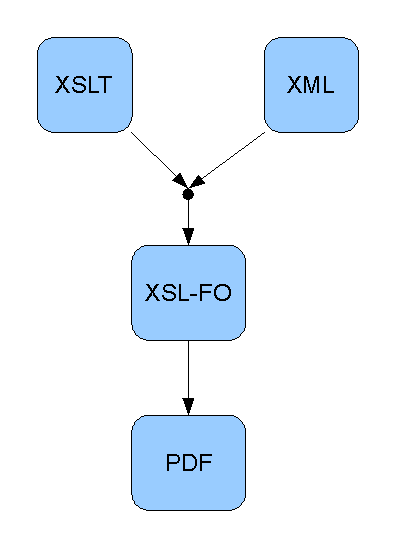
\includegraphics[width=0.30\textwidth]{Admin_PdfGenerierung.png}
	\caption{Pdf-Generierung}
	\label{Pdf-Generierung}
\end{figure}

Die XSLT Vorlagen werden in der Datenbank gespeichert und k�nnen pro Studiengang unterschiedlich sein.\\
Die zugeh�rige XML Datei wird von den Scripten im RDF Verzeichnis erstellt.\\
\\
\achtung{\textbf{Wichtig} Damit der Server die PDFs generieren kann, muss dieser ohne Authentifizierung auf das RDF-Verzeichnis zugreifen k�nnen.
Dies muss gesondert in den Einstellungen des Webservers eingetragen werden. \\
Ab Apache 2.2 kann dies auch per .htaccess eingestellt werden}\\

